\documentclass[a4paper,11pt]{article}
%\usepackage[utf8]{inputenc}
\usepackage[french]{babel}
\usepackage[T1]{fontenc}
\usepackage{amsmath}
\usepackage{graphicx}
\usepackage{enumitem}
\usepackage[lmargin=2.5cm,rmargin=2.5cm,tmargin=2cm,bmargin=2.5cm]{geometry}
\usepackage{listings}
\usepackage[dvipsnames]{xcolor}

\lstdefinestyle{mypython}{
    language=Python,
    backgroundcolor=\color{white},
    basicstyle=\ttfamily\footnotesize,
    frame=single,
    keywordstyle=\color{blue},
    commentstyle=\color{ForestGreen},
    stringstyle=\color{red},
    numbers=left,
    numberstyle=\tiny\color{gray},
    stepnumber=1,
    tabsize=4,
    showstringspaces=false
}

%\newenvironment{verbatim}{\begin{lstlisting}[style=mypython]}{\end{lstlisting}}
%\newenvironment{verbatim}{\begin{lstlisting}[style=mypython]}{\end{lstlisting}}

\setlength{\parindent}{0pt}

\newcounter{question}
\newcommand{\exequest}[1]{\bigskip \stepcounter{question} \textbf{Question \arabic{question}} : #1}

% Informations sur l'examen
\title{ENSAE TD noté, mercredi 6 novembre 2024}
\date{}

\begin{document}

\vspace{-3cm} 
\maketitle
\vspace{-1.5cm} 

\textit{L'accès à internet est autorisé mais l'utilisation d'intelligences artificielle génératives de type ChatGPT est interdite.}

\medskip
\emph{Toutes les questions valent 2 points.}
\bigskip

\begin{center}
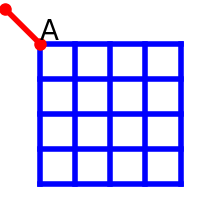
\includegraphics[width=0.25\textwidth]{td_note_2024.png}
\end{center}

25 maisons sont positionnées aux 25 intersections du quadrillage ci-dessus.
Le courant (rouge) arrive à un angle du carré (point A).
Il faut relier chaque maison au courant pour un coût minimal.
Pour cela il faut tirer un câble entre le point A et chaque intersection.
Les cibles ne peuvent passer que par les routes (les lignes du quadrillage),
pas de diagonales donc.

\emph{Les assertions du sujets (exprimées avec le mot clé \texttt{assert}) doivent être satisfaites par vos solutions.}

%%%%%
\exequest{Implémenter une fonction qui calcule la distance L1.}

La distance L1 est définie par $d(x_1,y_1,x_2,y_2) = |x_1 - x_2| + |y_1 - y_2|$.

\begin{lstlisting}[style=mypython]
def distance(x1, y1, x2, y2):
    # ...
    return ...

assert distance(0, 0, 3, 4) == 7
\end{lstlisting}

%%%%%
\exequest{Calculer la longueur de câble pour relier les 25 maisons.}

\begin{lstlisting}[style=mypython]
def longueur_cable(n=5):
    # ...

assert longueur_cable(5) == 100
\end{lstlisting}

On suppose dans la suite de l'énoncé que le quadrillage reste carré.

%%%%%
\exequest{Adapter la fonction pour un rectangle 8x9.}

\begin{lstlisting}[style=mypython]
assert longueur_cable(8, 9) == 540
\end{lstlisting}

%%%%%
\exequest{Avec deux câbles...}

On dispose de deux câbles : 

\begin{enumerate}
\item un câble ne pouvant relier qu'une maison avec un coût $c_1$ par mètre (un quadrillage $n\times m$ est de dimension $n$ mètres par $m$ mètres)
\item un câble ne pouvant relier qu'une ou deux maisons avec un coût $c_2$ par mètre
\end{enumerate}

Par conséquent, on peut relier une maison \textit{M1} avec un câble $c_2$ puis relier 
\textit{M1} à une autre maison \textit{M2} avec un câble $c_1$.
On veut savoir quand utiliser tel ou tel câble pour minimiser les coûts.

Ecrire une fonction qui retourne le coût du câblage décrit ci-dessus.

\begin{lstlisting}[style=mypython]
def cout_cablage(x1,y1, x2,y2, c1, c2):
    # ...

assert cout_cablage(1,2, 2,4, 1, 1.5) == 7.5
\end{lstlisting}

%%%%%
\exequest{Que fait le code suivant et que montre-t-il ?}

\begin{lstlisting}[style=mypython]
def position_m1(n, c1, c2):
    x = []
    y = []
    for i in range(2*n):
        x.append(i)
        y.append(cout_cablage(0,i, 0,n, c1, c2))
    return x, y

x, y = position_m1(5, 1, 1.5)
print(x)  # [0, 1, 2, 3, 4, 5, 6, 7, 8, 9]
print(y)  # [5.0, 5.5, 6.0, 6.5, 7.0, 7.5, 10.0, 12.5, 15.0, 17.5]
\end{lstlisting}

%%%%%
\exequest{Idée d'algorithme}

\begin{enumerate}
\item On prend une maison non câblée M1 la plus proche de A.
\item On prend ensuite une maison non câblée M2 la plus proche du coin opposé
\item On continue jusqu'à la fin.
\end{enumerate}

On crée une matrice $M$, $n \times n$ telle que $M[i][j]$ représente le numéro du câble ($1$ pour $c_1$ et $2$ pour $c_2$) qui relie la maison à l'intersection $i, j$ (sans information sur l'origine du cable). La maison 0, 0 est initialement reliée avec le câble 0, les autres valeurs sont initialisées à -1.

Écrire une fonction qui initialise la matrice.

\begin{lstlisting}[style=mypython]
def init(n=5):
    # ...
\end{lstlisting}

%%%%%
\exequest{Ecrire une fonction qui retourne la maison la plus proche d'une position $(i,j)$ et non câblée.}

\begin{lstlisting}[style=mypython]
def maison_proche(M, i, j):
    # ...

M = init()
assert maison_proche(M, 0,0) == (0, 1)
M[0][1] = 1
M[1][0] = 2
M[1][1] = 3
assert maison_proche(M,0,1) == (0, 2)
\end{lstlisting}


%%%%%
\exequest{On veut tirer un nouveau câble comme suit :}

\begin{enumerate}
\item on prend la maison $m_1$ la plus proche de A non cablée, on la cable avec le câble $c_2$
\item on met à jour la matrice M
\item on prend une maison proche du coin opposé (non câblée), qu'on cable avec $c_1$ depuis $m_1$
\item on met à jour la matrice M
\item on renvoie le coût de ces deux câbles ainsi que les deux maisons choisies
\end{enumerate}

Écrire une fonction qui tire un nouveau câble de cette manière :

\begin{lstlisting}[style=mypython]
def nouveau_cable(M, c1, c2):
   # ...

M = init()
g = nouveau_cable(M, 1, 1.5)
assert g == ((0, 1), (4, 4), 8.5)
\end{lstlisting}


%%%%%
\exequest{Terminer l'algorithme.}

Il suffit d'une boucle pour câbler toutes les maisons. La trouverez-vous ?

\begin{lstlisting}[style=mypython]
def algorithme_cablage(n, c1, c2):
    M = init(n)
    n_cables = n * n // 2
    cables = []
    # for ...
    # ...
    return cables

print(algorithme_cablage(5, 1, 1.5))
\end{lstlisting}


%%%%%
\exequest{L'algorithme a un défaut, trouverez-vous lequel ?}



\end{document}
